\documentclass{standalone}
% preamble: usepackage, etc.
  
\begin{document}
\chapter{Results and Discussion}
\label{Chapter4}
Image identification, classification, natural language processing, object detection, and segmentation, are the few problems that modern machine vision applications need answers to. Due to the inability of traditional machine learning to solve these complicated issue due to its strict coding constraints, deep learning approaches such as convolutional and recurrent neural networks have been introduced. It is important to mention that classical CNN models are data hungry and are unable to recognize object pose and location details, thereby prompting the development of capsule networks. 

The expectation of capsule networks in connection with all of the aforementioned problems, outperforms CNN models. Despite this promising performance, researchers are yet to fully exploit its advantages due to the lack of architectural information and understanding of the working principles of capsule network. Recently, some deep learning models are utilizing capsule networks as its primary back bone framework ever since it was introduced. The most widely used form of capsule network employs a layer-to-layer routing method known as "routing by agreement." In CNNs, this approach substitutes pooling and scalar outputs with a vector output. The size of the output denotes the probability that an attribute depicted by the capsule is present in the input, while the object's position denotes the instantiation variable.


%%%%%%%%%%%%%%%%%%%%%%%%%%%%%%%%%%%%%%%%%%%%%%%%%%%%%%%%%%%%%%%%%%%%%%%%%%%%%%%% Paper 2 %%%%%%%%%%%%%%%%%%%%%%%%%%%%%%%%%%%%%%%%%%%%%%%%%%%%%%%%%%%%%%%%%%%%%%%%%%%%%%%%%%%%%%%%%%%%%%%%

\textbf{\section{Shared Weighted Continuous Wavelet Capsule Network for Electrocardiogram Biometric Identification}} 

Despite various usability and security issues, conventional passwords remain the most used method of internet authentication [1]-[3]. Passwords are inconvenient for users since they must be remembered and preferably, be lengthy and distinct. As a result, it should come as no surprise that many users choose weak passwords that they reuse across several platforms [4], [5], resulting in account hack and personal data breaches. According to studies, over 50\% of users use the same authentication credentials for several platforms [4] and over 80\% of privacy breaches are caused by poor authentication credential behavior [6]. 

Alternative authentication techniques, such as push notifications [7], graphical passcodes [8], and trust scores [9], and gestures [10], have been investigated in attempt to replace or supplement standard passwords. Biometric authentication is of particular importance due to its unique characteristics of user identity. Biometrics enhances usability of the system by eliminating the need for users to remember passwords or move about with a token at all times. The simplicity with which biometrics can be used for authentication has sped up their adoption in both the private and public sectors, with the global market for biometric technology anticipated to hit \$59.31 billion by 2025 [11].

While much of the previous research has focused on standard biometrics like fingerprints, facial recognition, and iris scans, there has been little work done to investigate new biometrics. In this paper, we look at a biometric based on electrocardiogram (ECG) signals, which represent the electrical activity of the human heart. ECG has been shown to be adequately unique to every person in previous studies [12] and could be utilized for identity verification. In this paper, we proposed a hybrid scheme of continuous wavelet transform (CWT) and capsule network for biometric authentication based on ECG.CNN has made significant progress in a variety of applications, particularly in detecting anomalies in radiographs [13] – [16]. 

%\begin{figure*}[t!]
%\centering
%\includegraphics[scale=0.1]{C4/c4_p2-1}
%\caption{Proposed scheme for detecting DDoS attack on smart grid.}
%\label{fig:c4_p2-1}
%\end{figure*}

While biometrics are more usable than standard passwords, there are still issues about biometric data security and privacy [17]. Biometrics cannot be readily reversed once they have been infiltrated, as they are based on an individual's lasting physiological or behavioral features. Additionally, biometric recognition system operators may gain undesired information from a user's biometric data. Fingerprint patterns, for example, may be linked to certain disorders [18]. In conclusion, some biometric traits, such as a person's face, are difficult to conceal. As a result, even if a person wants to remain unknown, they may be recognized without their consent or knowledge [18].

The heart is a muscular organ that supplies blood to the body's tissues via blood vessels [19]. The heart muscle must contract in order to supply blood, resulting in an electrical impulse. During an electrocardiogram (ECG) examination, this impulse can be measured on the surface of the body using electrodes put on the skin. The process of depolarization and repolarization of the heart chambers, which causes them to contract and rest, is captured by an ECG tracing.

\begin{figure*}[t!]
\centering
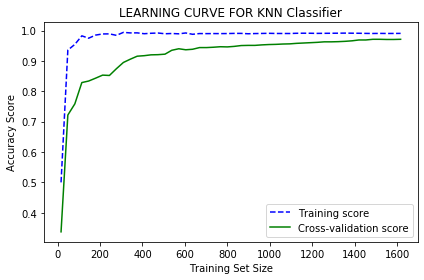
\includegraphics[scale=0.4]{C4/c4_p2-2}
\caption{Conversion of one-dimensional traffic data to two-dimensional images using CWT.}
\label{fig:c4_p2-2}
\end{figure*}

Various researchers have looked into the ECG's peculiarity and stability. The majority of these are based on a "on-the-person" approach "a method for signal acquisition in which electrodes are placed directly on the person [20]. There are limited researches that use "off-the-person" methodology "They use a different approach, but they show a real-life application scenario for ECG identification systems. Placing ECG sensors into a smartphone cover, wristbands, and car steering wheel are just a few instances. Additionally, as shown in [20], previous researches frequently employ data acquired from a single data acquisition session which are easy to develop. 

In this work, CWT is utilized to convert the 1-dimensional time-series signal of ECG to 2-dimensional time-frequency scalogram as input image of distinct features with growing sensitivity which makes it suitable for CNN model to extract feature for training. The image features obtained from CWT are utilized to train the proposed capsule network for biometric authentication. We adopted some well-known evaluation metrics to validate the performance of the proposed scheme. 
Conclusively, we assess the effectiveness of the proposed scheme using public dataset and also presented some comparison with other methods of biometric authentication.

\textbf{\subsection{Methodology}} 
The proposed method for biometric identification using ECG is described in this section. Figure 1 depicts the general framework of the proposed scheme for user identification. First, the dataset utilized in this study for ECG biometric identification is properly described. 

\textbf{\subsubsection{Dataset}} 

Instead of creating a new dataset, we used an already existed dataset. For this study, we used the MIT-BIH Normal Sinus Rhythm available on Physionet database. The Physionet MIT-BIH Normal Sinus Rhythm database consists of healthy ECG records of persons between the ages of 20 and 50 with no major arrhythmias collected at the Arrhythmia laboratory of Boston’s Beth Israel Hospital[21]. Compared to other ECG dataset, Physionet MIT-BIH dataset has been utilized by most studies. Physionet MIT-BIH dataset consists of 30 recordings of normal sinus rhythm signals.



\textbf{\subsubsection{Proposed siamese capsule network (WavCapNet)}} 

This research proposes a siamese capsule network, as shown in Figure 3. The model accepts two scalogram images as inputs, and then transmits them into a shared weighted framework. The obtained data is forwarded into the fully-connected layer, and the model then determines if the outcome is valid or invalid. Our proposed model's method is based on a real-world security assessment of person identity.

In a real-world scenario, tenants of a specific building or employees of a company with access control security equipment are normally asked to go through a security check. These persons' biometric templates must have been stored in the system. When a person attempts to enter an authorized building or organization, a comparison of both the template and the query input is performed to determine whether the request is valid or invalid. As a result, the idea of employing a siamese capsule network to receive both ECG trait images, access their attributes, and determine whether they are similar or not is proposed. In general, a siamese network is used to compare two input images with similar weights and parameters. The extracted feature vectors of the two inputs are then obtained from the last layer, and the Euclidean distance is computed. If the distance between the two images is large, they are different, otherwise, they are similar.


Computing the similarity of the ECG images will be omitted in our investigation, and instead the relationship between the two images will be utilized to predict the outcome. As a result, the distance calculating aspect of our work is eliminated, as shown in Figure 3. For feature extraction, a shared weighted capsule network with modified AlexNet as the base neural network is used, then the retrieved features are fused and passed into the fully-connected layer, and ultimately, the ECG images are predicted using a sigmoid classifier. Instead of the usual max-pooling layer, we introduced discrete wavelet pooling to replace the first and second max-pooling layers for down-sampling operation whereas the third max-pooling layer is eliminated to arrive at a feature vector of $256 \times 14 \times 14 $. The likelihood of which ECG trait matches the query or not is represented by the prediction result which is either 0 or 1.

\textbf{\subsubsection{Experimental detail and setup}} 

The basic technique of the proposed scheme is split into two phases: data pre-processing and feature extraction. The pre-processing step begins with the collection of raw ECG signals from the Physionet database. The most essential and consistent fundamental characteristics are obtained in the pre-processing step by converting one-dimensional time domain ECG signal to time-frequency domain image of two-dimension using CWT. This work employed continuous wavelet transform and siamese wavelet capsule networks trained on Physionet MIT-BIH ECG dataset for biometric identification using Adam optimizer and dropout to prevent over-fitting, early stop strategies, and a learning rate of $10^{4}$ to improve performance. Keras library with Tensorflow as the backend on a GeForce GTX 1080 GPU is used for the implementation of this work. Accuracy, sensitivity, specificity and AUC are some of the evaluation metrics applied on our proposed model. 

\begin{table}[]
\caption{Performance comparison of our proposed model with selected pre-trained models.
WavCovNet model.}
\begin{tabular}{lllll}
\toprule
\multicolumn{1}{l}{Model} & \multicolumn{1}{l}{ACC (\%)} & \multicolumn{1}{l}{SEN (\%)} & \multicolumn{1}{l}{SPE (\%)} & \multicolumn{1}{l}{Time (Min)} \\ \hline
\midrule
ResNet-101                  & 95.7                         & 95.8                         & 94.6                         & 47                              \\
EfficientNet                & 94.7                         & 94.3                         & 95.8                         & 40                              \\
MobileNet-V3                & 95.2                         & 94.5                         & 95.9                         & 39                              \\
DenseNet                    & 96.6                         & 95.4                         & 96.3                         & 46                              \\ 
\multicolumn{1}{l}{Ours}  & \multicolumn{1}{l}{99.2}    & \multicolumn{1}{l}{98.6}    & \multicolumn{1}{l}{99.5}    & \multicolumn{1}{l}{48}         \\ \hline
\bottomrule
\end{tabular}
\label{tab6}
\end{table}



\textbf{\subsubsection{Results and discussion}} 
The proposed ECG biometric identification scheme is built using the Keras framework and Tensorflow as the backend. We examined the proposed strategy for ECG biometric identification based on binary classification for both query match and mismatch in security access control systems during training and validation. The proposed approach obtains 99.2\% accuracy rate for identifying query match and mismatch. The proposed model's training and validation accuracy curves are depicted in Figure 4, which show that the model converges smoothly without over-fitting. The proposed scheme's training and validation loss curves are gradually and steadily reduced as shown in Figure 5. In general, the proposed siamese wavelet capsule network's performance is reasonable. It's crucial to evaluate the proposed model's validity using the receiver operating characteristic curve (ROC), which depicts the proposed scheme's overall accuracy in terms of area under the curve (AUC). Figure 6 illustrates that the proposed scheme has a high sensitivity combined with a high specificity, resulting in a low false positive rate and a high true positive rate.



As shown in Table 1, our proposed approach obtains 98.6\% sensitivity and 99.5\% specificity. The results of our proposed scheme versus certain pre-trained models are shown in Table 1. When it comes to correctly determining query match and mismatch of ECG characteristics, the proposed strategy clearly outweighed the selected pre-trained techniques by 2.6\% in terms of accuracy. In addition, the proposed method achieved 2.6\% increase in sensitivity and 3.2\% increase in specificity when compared to pre-trained procedures. EfficientNet had the lowest accuracy (94.7\%) and sensitivity (94.3\%) scores, whereas ResNet-101 had the lowest specificity score (94.6\%). It is worth noting that the proposed scheme has a slightly higher computational time of about 48 minutes in training but achieves the best result, as shown in Table 1. Though MobileNet-V3 had the shortest training time of 39 minutes, our proposed model still achieves satisfactory performance. 

\textbf{\subsubsection{Conclusions}} 

Biometric identification systems provide several benefits that traditional techniques do not. We proposed an ECG-based biometric identification system for security access control in this research, in which a continuous wavelet transform (CWT) was utilized to convert one-dimensional time-domain signals into scalograms of two-dimensional images to obtain good quality training data. A siamese capsule network framework was utilized to predict the right match or mismatch of ECG query samples using the extracted specific attributes from the scalograms. The findings show that the ECG signal is a reliable biometric measure that is resistant to noise and artifacts. Furthermore, the proposed security system's efficiency was assessed using both classification metrics and the ROC-AUC measure. The proposed scheme properly predicted ECG query samples with 99.2\% accuracy, which is 2.6\% higher than the other models.





%%%%%%%%%%%%%%%%%%%%%%%%%%%%%%%%%%%%%%%%%%%%%%%%%%%%%%%%%%%%%%%%%%%%%%%%%%%%%%%%%%%%%%%%%%%%%%%%%%%%%%
\end{document}